\chapter{TINJAUAN PUSTAKA}

\section{Kajian Penelitian}

Penelitian yang dilakukan dalam pembuatan sistem deteksi, ekstraksi,
dan penghitungan luas batu ginjal menggunakan gabungan YOLO dan pengolahan
citra ini dilakukan dengan mempelajari penelitian-penelitian yang
sudah dilakukan oleh peneliti terdahulu. Penelitian yang dikaji mengutamakan
penelitian seputar deteksi batu ginjal dengan menggunakan model algoritma
\emph{machine learning} You Only Look Once (YOLO) dan perhitungan
luas batu ginjal tersebut dengan pendekatan pengolahan citra.

\subsection{\emph{Real-Time Object Detection in Medical Imaging Using YOLO Models
for Kidney Stone Detection} \citep{billah12s}}

Penelitian ini membahas deteksi batu ginjal secara real-time menggunakan
model YOLOv8 dan YOLOv10 pada citra CT \emph{scan} medis.

\vspace{20pt}

Tabel 2.1 menjelaskan secara ringkas penelitian-penelitian terdahulu
terhadap deteksi, ekstraksi, dan penghitungan luas batu ginjal menggunakan
gabungan YOLO dan pengolahan citra yang sudah dikaji.

\vspace{-10pt}

\begin{table}[H]
\begin{spacing}{0}
\caption{Rangkuman Penelitian Terdahulu}
\end{spacing}
\end{table}

\vspace{-20pt}
\begin{center}
\begin{longtable}[c]{|>{\centering}m{0.5cm}|>{\raggedright}p{3cm}|>{\raggedright}p{3.5cm}|>{\raggedright}p{5cm}|}
\hline 
\centering{}{\footnotesize\textbf{No}} & \centering{}{\footnotesize\textbf{Peneliti}} & \centering{}{\footnotesize\textbf{Judul Penelitian}} & {\footnotesize\textbf{Hasil}}\tabularnewline
\endfirsthead
\hline 
\centering{}{\footnotesize\textbf{No}} & \centering{}{\footnotesize\textbf{Peneliti}} & \centering{}{\footnotesize\textbf{Judul Penelitian}} & {\footnotesize\textbf{Hasil}}\tabularnewline
\endhead
\hline 
{\footnotesize 1} & {\footnotesize\citealp{billah12s}} & {\footnotesize\emph{Real-Time Object Detection in Medical Imaging
Using YOLO Models for Kidney Stone Detection}} & {\footnotesize Hasil menunjukkan bahwa YOLOv10 unggul dalam akurasi
(91\% dibandingkan 88\% untuk YOLOv8)}\tabularnewline
\hline 
 &  &  & \tabularnewline
\hline 
 &  &  & \tabularnewline
\hline 
 &  &  & \tabularnewline
\hline 
 &  &  & \tabularnewline
\hline 
 &  &  & \tabularnewline
\hline 
 &  &  & \tabularnewline
\hline 
\end{longtable}
\par\end{center}

\vspace{-40pt}

\section{\emph{Flowchart}}

Secara formal, \emph{flowchart} adalah representasi diagramatik dari
langkah-langkah suatu algoritma. Dalam \emph{flowchart}, digunakan
kotak dengan bentuk berbeda untuk menunjukkan jenis operasi yang berbeda.
Kotak-kotak ini kemudian dihubungkan oleh garis dengan panah yang
menunjukkan aliran atau arah yang harus diikuti untuk mengetahui langkah
selanjutnya. Garis penghubung ini dikenal sebagai garis alir (\emph{flow
line}).

\emph{Flowchart} program adalah alat yang sangat berguna dalam pengembangan
program. Pertama, kesalahan atau kelalaian dapat lebih mudah dideteksi
dari \emph{flowchart} program daripada dari program itu sendiri karena
\emph{flowchart} program adalah representasi bergambar dari logika
program. Kedua, \emph{flowchart} program dapat diikuti dengan mudah
dan cepat. Ketiga, ini berfungsi sebagai dokumentasi, yang dapat sangat
membantu jika diperlukan modifikasi program di masa mendatang.

\emph{Flowchart} dapat digunakan untuk menunjukkan urutan langkah
untuk melakukan pekerjaan apa pun. Rangkaian operasi sederhana yang
melibatkan penerimaan \emph{input}, pelaksanaan operasi aritmetika
pada \emph{input}, dan menampilkannya kepada pengguna dapat digunakan
untuk menunjukkan struktur logika sekuensial dari suatu program \citep{chaudhuri2020flowchart}.

\begin{table}[H]
\caption{Simbol Standar \emph{Flowchart} Program}

\centering{}(Sumber: \citealp{chaudhuri2020flowchart})
\end{table}

\vspace{-25pt}

\begin{longtable}[c]{|>{\centering}m{4cm}|>{\raggedright}m{9.5cm}|}
\hline 
\textbf{Simbol} & \centering{}\textbf{Keterangan}\tabularnewline
\hline 
\endfirsthead
\hline 
\textbf{Simbol} & \centering{}\textbf{Keterangan}\tabularnewline
\hline 
\endhead
\hline 
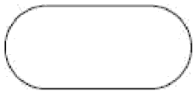
\includegraphics[totalheight=1.3cm]{images/flow_terminal} & Terminal:

Digunakan untuk menunjukkan awal dan akhir dari rangkaian proses yang
berhubungan dengan komputer.\tabularnewline
\hline 
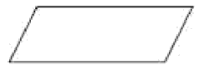
\includegraphics[totalheight=1cm]{images/flow_io} & \emph{Input/Output} (Masukan/Keluaran):

Digunakan untuk menunjukkan operasi \emph{input/output} apa pun.\tabularnewline
\hline 
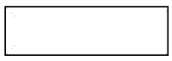
\includegraphics[totalheight=1cm]{images/flow_proc} & Pemrosesan Komputer (\emph{Computer Processing}):

Digunakan untuk menunjukkan pemrosesan apa pun yang dilakukan oleh
sistem komputer.\tabularnewline
\hline 
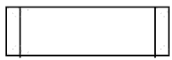
\includegraphics[totalheight=1cm]{images/flow_predproc} & Pemrosesan Tertentu (\emph{Predefined processing}):

Digunakan untuk menunjukkan proses apa pun yang tidak didefinisikan
secara khusus dalam \emph{flowchart}.\tabularnewline
\hline 
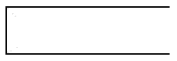
\includegraphics[totalheight=1cm]{images/flow_comm} & Komentar (\emph{Comment}):

Digunakan untuk menulis pernyataan penjelasan yang diperlukan untuk
memperjelas sesuatu.\tabularnewline
\hline 
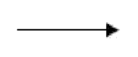
\includegraphics[totalheight=1.5cm]{images/flow_fl} & Garis Alir (\emph{Flow line}):

Digunakan untuk menghubungkan simbol-simbol \emph{flowchart}.\tabularnewline
\hline 
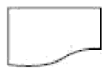
\includegraphics[totalheight=1.5cm]{images/flow_docio} & Masukan/Keluaran Dokumen (\emph{Document Input/Output}):

Digunakan ketika \emph{input} berasal dari dokumen dan \emph{output}
menuju ke dokumen.\tabularnewline
\hline 
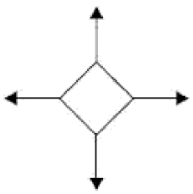
\includegraphics[totalheight=1.8cm]{images/flow_deci} & Keputusan (\emph{Decision}):

Digunakan untuk menunjukkan titik mana pun dalam proses di mana keputusan
harus dibuat untuk menentukan tindakan selanjutnya.\tabularnewline
\hline 
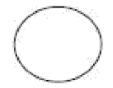
\includegraphics[totalheight=1.7cm]{images/flow_oncon} & Penghubung Halaman (\emph{On-page Connector}):

Digunakan untuk menghubungkan bagian-bagian \emph{flowchart} yang
dilanjutkan pada halaman yang sama.\tabularnewline
\hline 
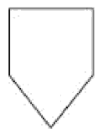
\includegraphics[totalheight=1.9cm]{images/flow_offcon} & Penghubung Antar-Halaman (\emph{Off-page Connector}):

Digunakan untuk menghubungkan bagian-bagian \emph{flowchart} yang
dilanjutkan ke halaman yang terpisah.\tabularnewline
\hline 
\end{longtable}